\section{Exiperments and Evaluation}\label{sec:evaluation}
%\subsection{Exiperments}
\par  To evaluate the effectiveness of our method, a Spark cluster with 4 nodes (one master node and three slave node) is deployed. The master node has Xeon processor E3-1200 v3 and 128GB memory. All slave nodes were with eight 3.40 GHz In-tel Core i7 and 8GB memory. Each node has also the same software stack: Ubuntu 16.04 LT and Spark 2.2.0 with Hadoop 2.7.3. 
\par We select WordCount and Sort benchmarks respectively. The iterations of algorithm is 100. The population number is 40. In order to get fast running , we set a threshold $T$, which represents difference degree in the between particles.  The value range of $T$ always between 0 and 0.1. If the threshold value is too big,  the particle will not reach the best position. If the threshold value is too small, the particle will enter the local optimization. And we select twenty-two main parameters, which are shown in Table~\ref{tab:parameters}. Our motivation for choosing these benchmarks is as follows. First, these workloads are simple and easy to understand. Secondly, these benchmarks are representative of real Spark applications, with a wide range of applications. Finally, these benchmarks cover different application types, including I/O intensive, CPU intensive, memory-intensive, and iterativeintensive.
\par We adopt the Sort benchmark first, and get some results as follows. 
\begin{figure}[!htbp]
	%\vspace{-3mm}
	\centering
	\subfigure[The optimization solution when T and N take different values.]
	%\label{fig:sortrunning}
	{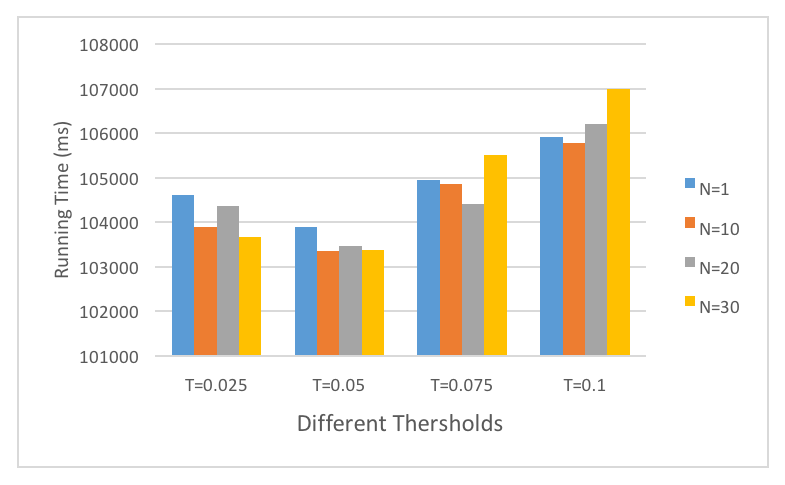
\includegraphics[width=0.48\linewidth]{SortRunningTime.eps}}
	\subfigure[The iterations when T and N take different values.]
	%\label{fig:sortiterations}
	{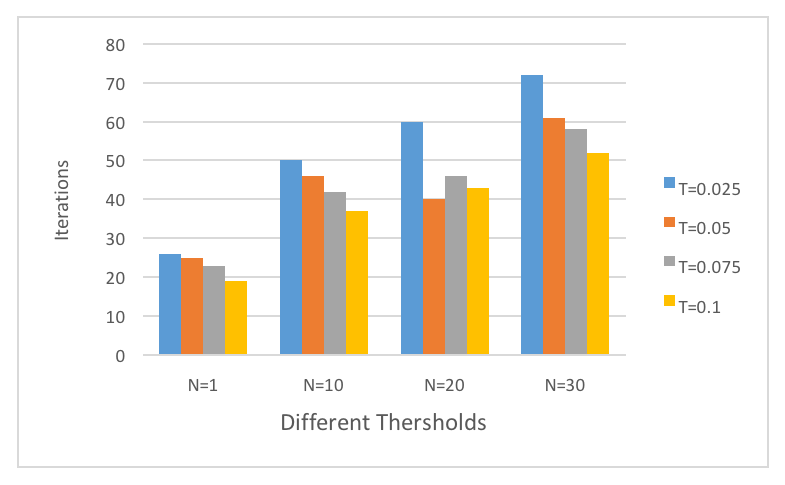
\includegraphics[width=0.48\linewidth]{SortIterations.eps}}\\
	\centering
	\caption{Experiment Results in Sort Benchmark.}
	\vspace{5mm}
	\label{fig:sortcompare}
\end{figure}
\par From above the Figure 6a and Figure 6b, respectively, for $T$ and $N$ take different values, the input 1.6 GB dataset to obtain the optimal solution and algorithm to obtain the optimal solution required for the number of iterations. When $T$ = 0.025 and $N$= 20, the optimal solution is 104,371 ms and the number of iterations is 60. When $T$ = 0.05 and $N$ = 10, the suboptimal solution is 103,360 ms and the number of iterations is 46. In contrast, the optimal solution efficiency is lower by 0.02\%, but the number of iterations is less than 38.68\%. Therefore, when the number of iterations and the optimal solution is taken into account, the algorithm can reach the time of best search status when A = 0.05 and N = 10. 
\par Now we address the Wordcount benchmark. Because the wordcount program has different steps, So we got the following results.
\begin{figure}[!htbp]
	%\vspace{-3mm}
	\centering
	\subfigure[The optimization solution when T and N take different values.]
	%\label{fig:wordcountrunning}
	{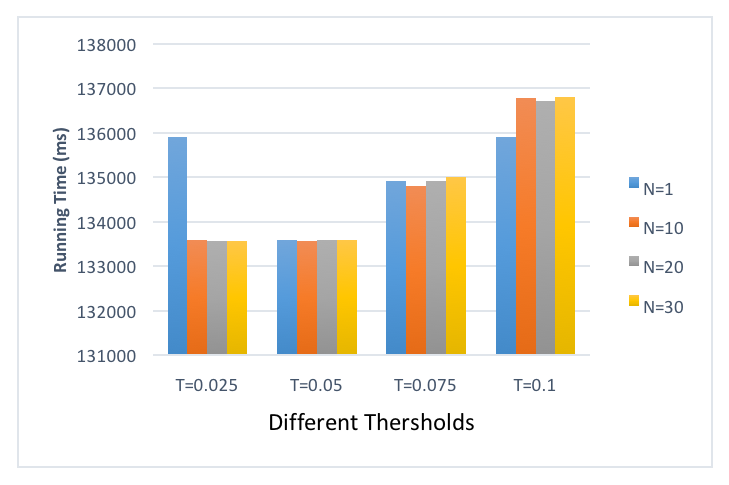
\includegraphics[width=0.48\linewidth]{wordcountRunningTime.eps}}
	\subfigure[The iterations when T and N take different values.]
	%\label{fig:wordcountiterations}
	{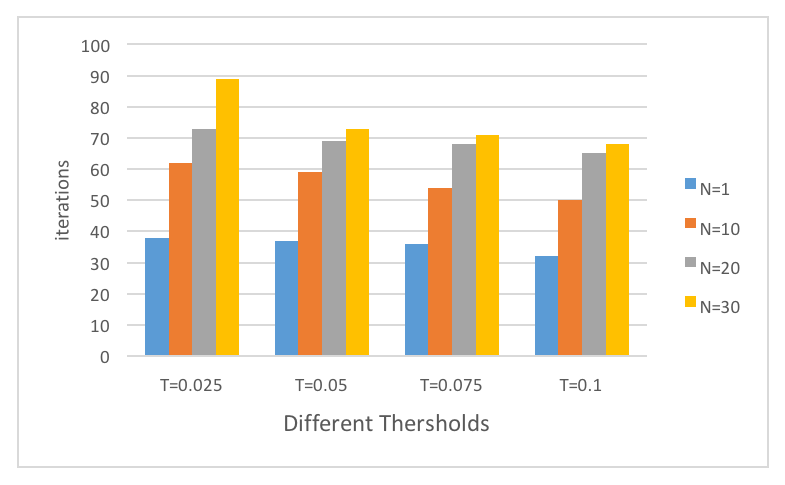
\includegraphics[width=0.48\linewidth]{wordcountIterations.eps}}\\
	\centering
	\caption{Experiment Results in Wordcount Benchmark.}
	\vspace{5mm}
	\label{fig:wordcountcompare}
\end{figure}
\par From above the Figure 7a and Figure 7b, respectively, for $T$ and $N$ take different values, the input 1.6 GB dataset to obtain the optimal solution and algorithm to obtain the optimal solution required for the number of iterations. When $T$ = 0.025 and $N$= 30, the optimal solution is 133,583 ms and the number of iterations is 73. When $T$ = 0.05 and $N$ = 10, the suboptimal solution is 133,560 ms and the number of iterations is 59. In contrast, the optimal solution efficiency is lower by 0.018\%, but the number of iterations is less than 36.63\%. Therefore, when the number of iterations and the optimal solution is taken into account, the algorithm can reach the time of best search status when A = 0.05 and N = 30.
%\begin{figure}
%   \centering
%  \begin{subfigure}[b]{0.5\textwidth}
%        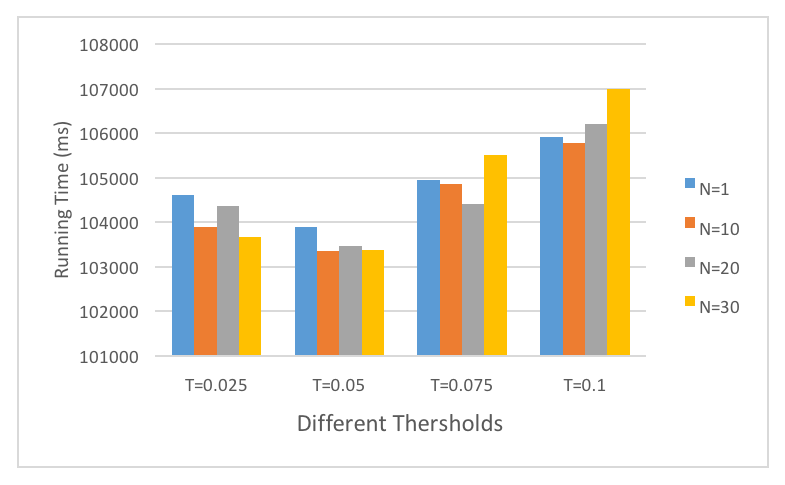
\includegraphics[width=\textwidth]{SortRunningTime.eps}
%        \caption{The optimization solution when T and N take different values}
%        \label{fig:gull}
%    \end{subfigure}
    ~ %add desired spacing between images, e. g. ~, \quad, \qquad, \hfill etc. 
      %(or a blank line to force the subfigure onto a new line)
%    \begin{subfigure}[b]{0.5\textwidth}
%        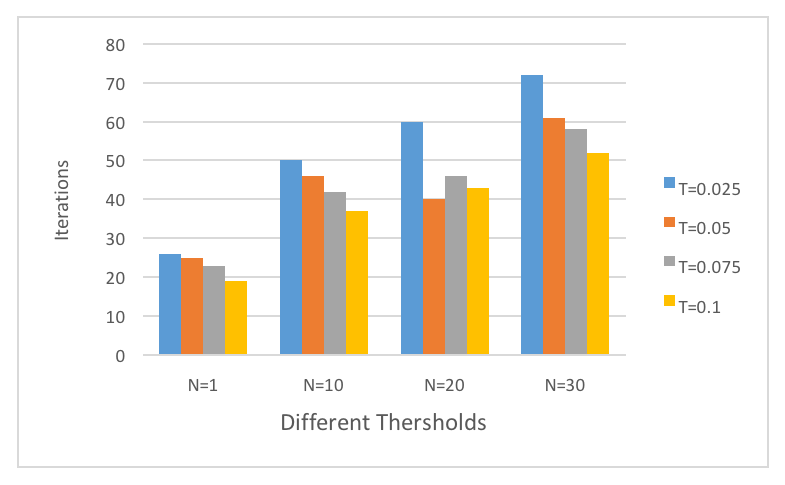
\includegraphics[width=\textwidth]{SortIterations.eps}
%        \caption{The iterations when T and N take different values}
%        \label{fig:tiger}
%    \end{subfigure}
    ~ %add desired spacing between images, e. g. ~, \quad, \qquad, \hfill etc. 
    %(or a blank line to force the subfigure onto a new line)
%    \caption{Experiments in Sort Benchmark}\label{fig:sortcompare}
%\end{figure}

\par Table \ref{tab:runningtimecompare} for the selection of the same size of 20 different input data experiments, respectively, in the default configuration and our proposed approach to find the optimal configuration run under the average running time. It can be seen that compared with the default configuration scheme, the configuration efficiency of the system can be greatly improved by the our proposed approach, and the operation efficiency is more obvious when the input data of job is larger. 
\begin{table}[htbp!]
\centering
\caption{Running Time of Job between Defalut and Optimization.} \label{tab:runningtimecompare} 
\begin{center}
    \begin{tabular}{l*{2}{c}r}
    \hline
    Configuration & Job 0.8GB & Job 1.6GB & Efficiency(\%) \\
    \hline
    Defalut & 10,675ms & 21,873ms & 28.6 \\
    Optimization & 7,952ms & 14,626ms & 18.9  \\
    \hline
    \end{tabular}
\end{center}
\end{table}

\par   In the other words, we can say our proposed approach is very suit for big data analysis system. Such as Spark platform. It has a good robustness and stability.
